\part{Entwurfsentscheidungen}

\section{Einleitung}
Dieses Dokument beschreibt den Entwurf des Programms "Datenflussanalyse zum Durchklicken". Es ist nach dem Top-Down-Prinzip aufgebaut. 
Zunächst werden in diesem einführenden Abschnitt unsere Entwurfsentscheidungen beschrieben und die Beweggründe, auf welchen diese beruhen, näher erläutert.
Es wird eine Übersicht über alle Pakete gegeben und die Aufgaben der verwendeten externen Libraries werden beschrieben. 
Anschließend folgt eine detaillierte Beschreibung aller Klassen und die Erklärung aller öffentlichen Methoden. 
Wichtige private Attribute werden genannt, um die Vollständigkeit zu gewährleisten und um die Funktionen öffentlicher Methoden zusammenhängend erklären zu können. 
Im Anschluss werden Sequenzdiagramme der wichtigsten Funktionen des Programms gezeigt, Änderungen in Bezug auf das Pflichtenheft aufgelistet und ein vollständiges Klassendiagramm aller Klassen angehängt.

\section{Architektur}
Bei diesem Entwurf wird das Model-View-Controller (MVC) Architekturmuster verwendet. 
Diese Entwurfsentscheidung erleichtert die spätere Weiterentwicklung und die Erweiterung des Programms mit weiterer Funktionalität. \par
Das Modell dieser Architektur beinhaltet die darzustellenden Daten und die erforderliche Logik für die Funktionalität des Programms. 
Die Präsentationsschicht beinhaltet die für die Darstellung und die Interaktion mit dem Benutzer notwendigen Daten. Die Steuerung ist für die Umsetzung der vom Benutzer geforderten Änderungen/Funktionalität zuständig. 
Sie wird durch die Benutzerinteraktion angesprochen und informiert das Modell über die zu ändernden Daten oder notwendigen Vorgänge.

\section{Modulübersicht}
Der Entwurf setzt sich aus den in der folgenden Graphik dargestellten Modulen gemäß dem MVC-Muster zusammen.
Dabei gehören das DFAFramework-Modul, das Analysen-Modul, das CodeProcessor-Modul und das Reflections-Modul zum Model. 
Der View wird durch das GUI-Modul, das VisualGraph-Modul und das JGraphX-Modul gebildet. \par
Das DFAFramework liefert die Logik für die Funktionalität des Programms. 
Es benutzt dabei das Analyse-Modul, in welchem sich die von uns implementierten Datenflussanalysen befinden. 
Diese Datenflussanalysen implementieren ein zentrales Interface des DFAFrameworks. 
Des Weiteren ist es abhängig von den externen Libraries Soot und Reflections (siehe unten). 
Der Controller ist für die Kommunikation zwischen dem DFAFramework und dem User Interface zuständig. 
Dabei benutzt er das InputProcessor-Modul, welches zwischen dem Controller und Soot vermittelt. 
Durch diesen Input-Prozessor ist der Controller weitestgehend unabhängig von der verwendeten Library Soot. \par 
Das GUI-Modul ist für die Darstellung der Information und für die Interaktion mit dem Benutzer zuständig. 
Dabei verwendet es das VisualGraph-Modul, welches für die Kommunikation zwischen der logischen Struktur des DFAFrameworks und der visuellen Information im \inlinecode{VisualGraphPanel} inklusive der Interaktion des Benutzers mit diesem verantwortlich ist. 
Das VisualGraph-Modul verwendet die Libary JGraphX und ist ebenfalls für den Export von Graphen verantwortlich.

\begin{figure}[htbp] 
  \centering
     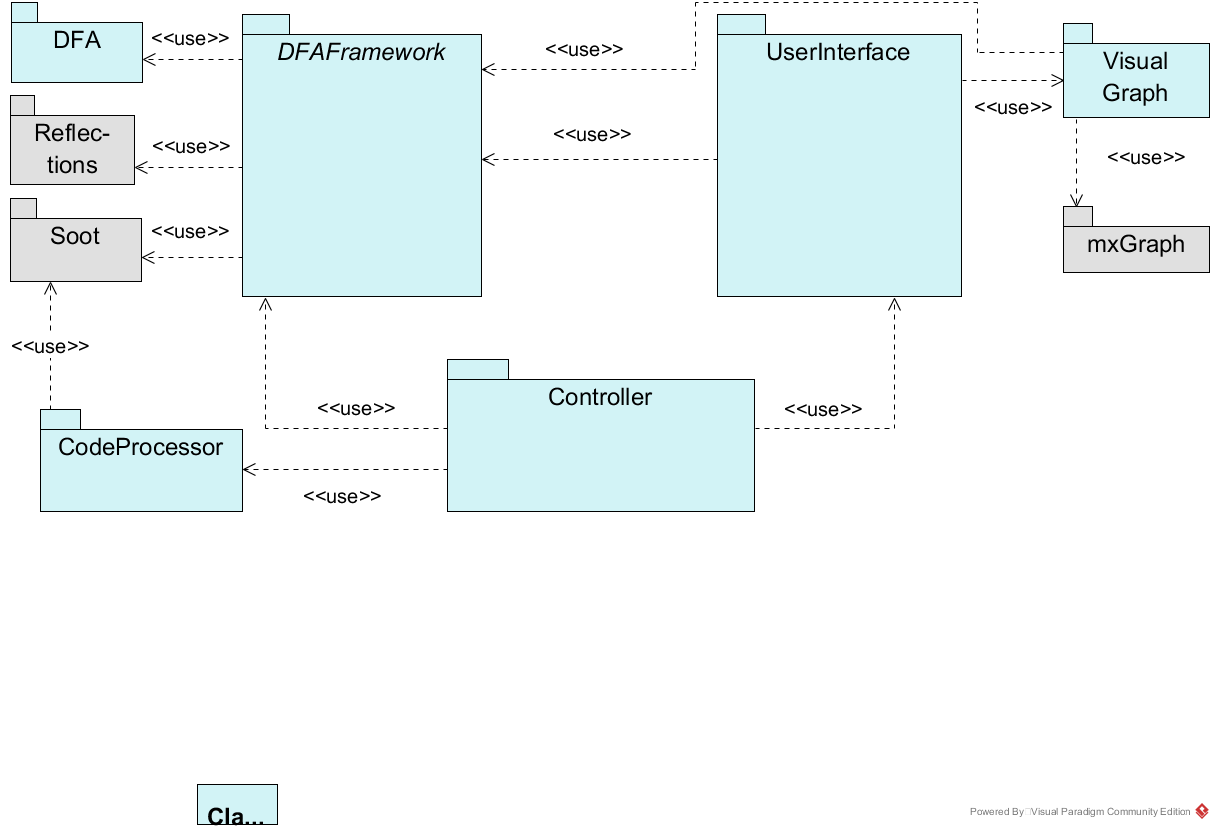
\includegraphics[width=1\textwidth]{Entwurfsentscheidungen/PackageOverview}
  \caption{Modulübersicht}
  \label{fig:Ubersicht}
\end{figure}

\newpage
\section{Externe Libraries}

\subsection{JGraphX}

JGraphX (\url{https://github.com/jgraph/jgraphx}) ist eine Java-Library zum automatischen Layouten und zum Zeichnen von Graphen. 
Damit eignet sich JGraphX gut, um den im Rahmen der Animation von Datenflussanalysen erstellten Kontrollflussgraphen zu visualisieren. Insbesondere bietet JGraphX die Möglichkeit, Knoten weiter in Zellen (\lstinline{mxCell}) zu unterteilen.
Dies ermöglicht die zeilenweise Animation der Datenflussanalysen.

\subsection{Reflections}

Reflections (\url{https://github.com/ronmamo/reflections}) ist eine Java-Library, die es erlaubt, zur Laufzeit neue Java-Klassen zu laden, sowie Metainformation über diese zu erhalten.
Dies wird dazu benutzt, um zur Laufzeit neue Datenflussanalysen zu laden.
Dazu wird ein festgelegter Ordner bei Programmstart auf kompilierte Java-Dateien (.class-Dateien) aus einem bestimmten Package [?! noch festlegen !?] untersucht. 
Dann werden alle Klassen, die von \lstinline{DataFlowExecution} erben, geladen und als Datenflussanalysen bereitgestellt. 


\subsection{Soot}

Soot (\url{https://github.com/Sable/soot}) ist eine Java-Library, die viele Funktionalitäten für statische Programmanalysen bereitstellt. 
Insbesondere bietet Soot mehrere Zwischencode-Formate an, in die gegebener Java-Bytecode übersetzt werden kann. 
In diesem Projekt wird Jimple als Zwischencode verwendet, auf dem die Datenflussanalysen erfolgen.
Bei Jimple handelt es sich um einen Expression-basierten typisierten Drei-Adress-Code.
Die elementaren Codeeinheiten sind also Expressions (Ausdrücke), die jeweils maximal drei Operanden haben.
Neben einer Zwischencode-Repräsentation bietet Soot die Möglichkeit, einen Kontrollflussgraphen aus Java-Bytecode zu erzeugen.
Die Grundblöcke des erzeugten Kontrollflussgraphen enthalten dann entsprechenden Zwischencode (hier Jimple).